\chapter{Application}
\section{Architecture}

\begin{figure}[h!]
  \centering
      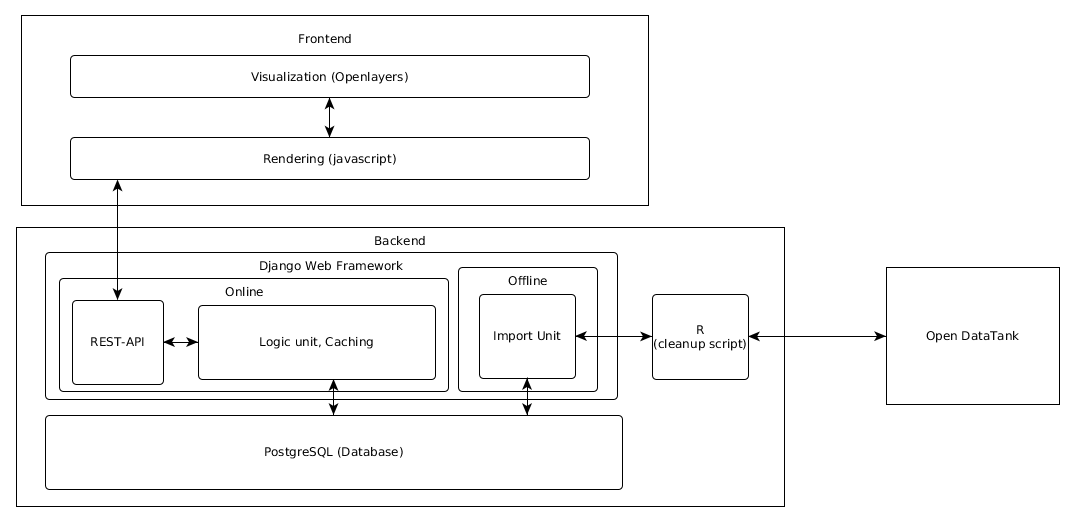
\includegraphics[width=16cm]{fig/Architecture}
 	 \caption{The final architecture of our web application}
\end{figure}
\subsection{Frontend}


\begin{figure}[h!]
	\centering
	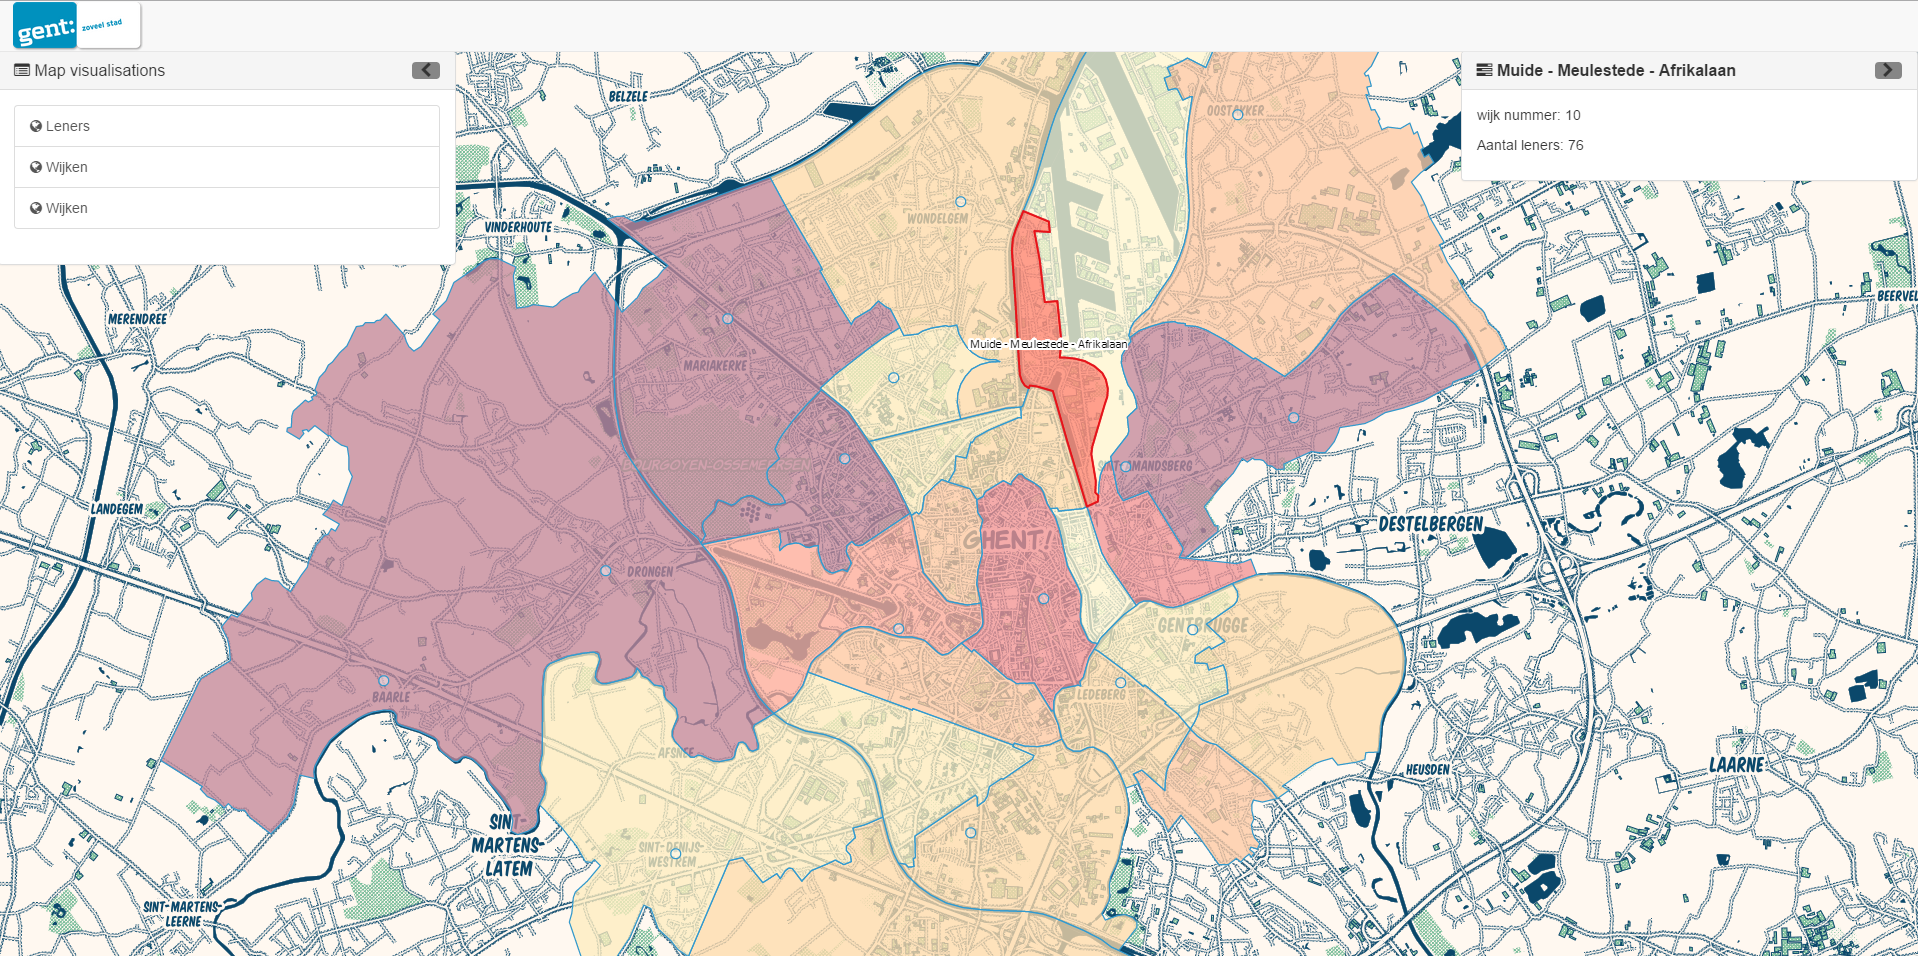
\includegraphics[width=16cm]{fig/frontend}
	\caption{Preview of the frontend, when you click on a certain neighbourhood on the interactive map}
	\label{fig:frontend}
\end{figure}

\begin{figure}[h!]
	\centering
	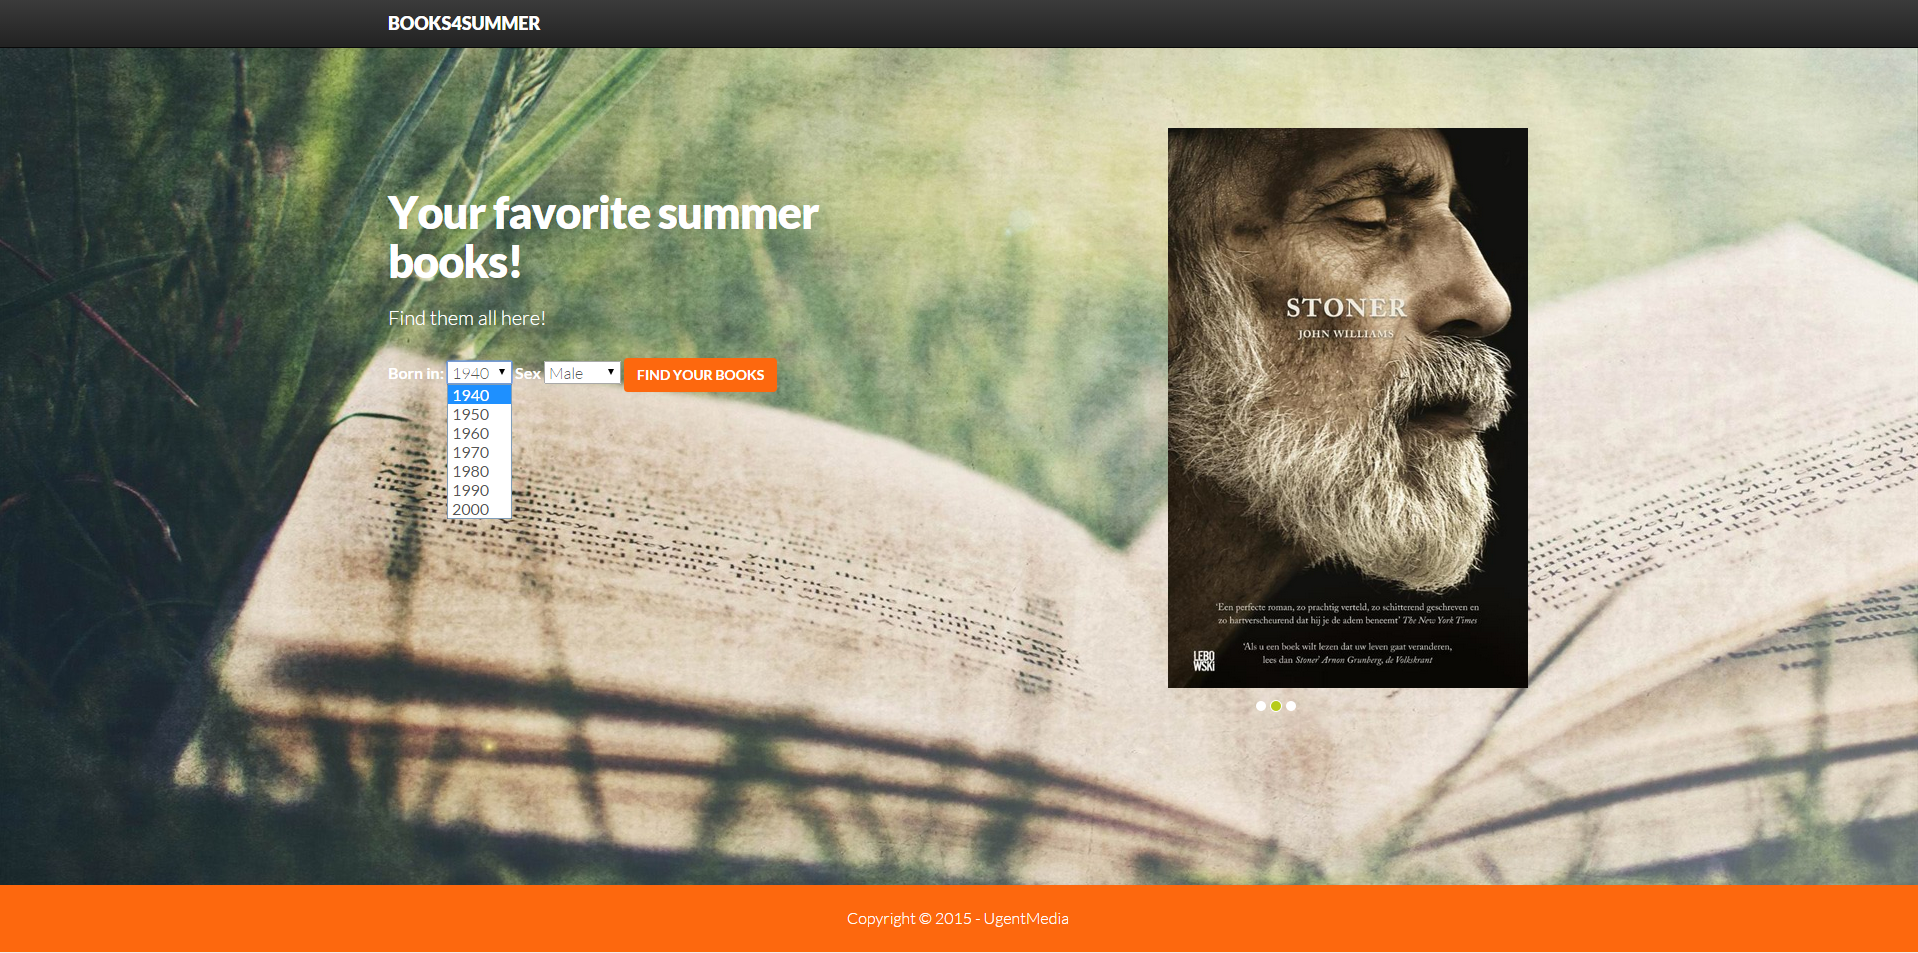
\includegraphics[width=16cm]{fig/books4summer}
	\caption{A website for the journalists with the list of the most borrowed books in summer based on selected criteria.}
	\label{fig:books4summer}
\end{figure}


\begin{figure}[h!]
	\centering
	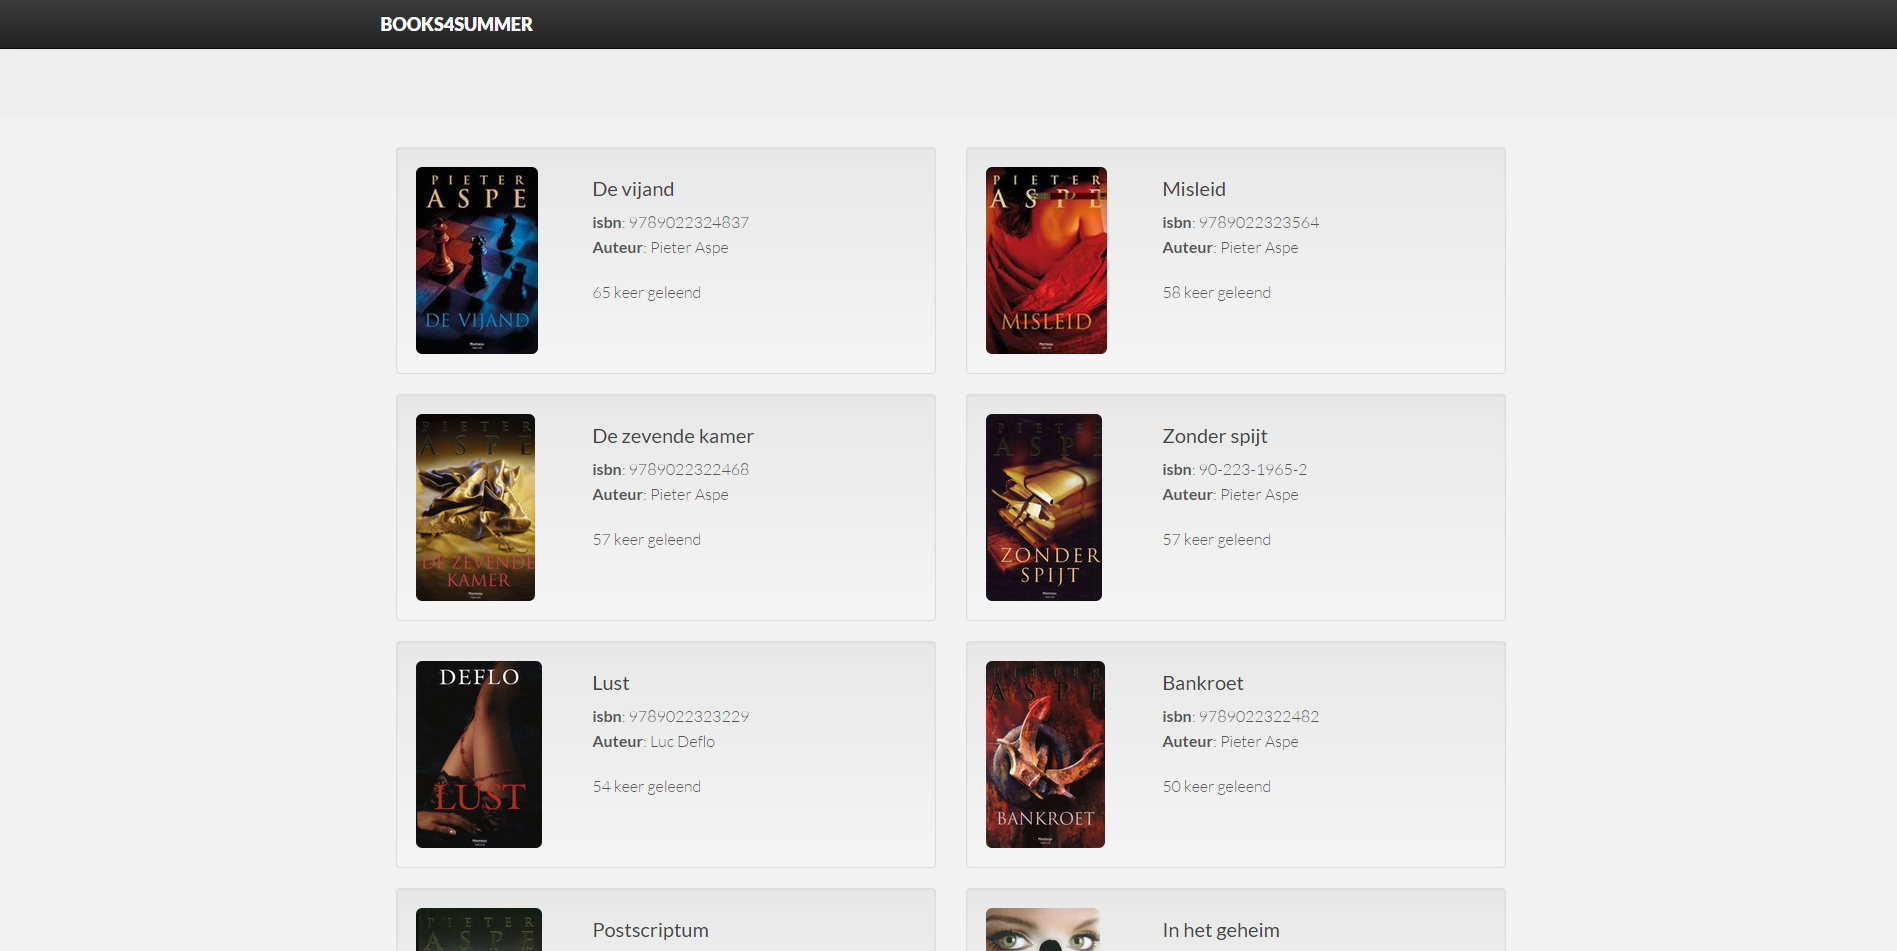
\includegraphics[width=16cm]{fig/books4summer-result}
	\caption{Example of the most borrowed books in summer 2009-2014 for men born in 1940's.}
	\label{fig:books4summer-result}
\end{figure}

At the frontend side of our web application (Fig.~\ref{fig:frontend}), we will have two main components, a rendering component and a visualization component. At the rendering block, the data requested via the API from the backend will be transformed into e.g. figures, dots, that can be displayed on the browser. When the transformation is finished, the visualization block will show the transformed data on the website itself.\\
An additional website (Fig.~\ref{fig:books4summer}) that uses the library data was made for the journalists. It presents the most borrowed books in summer 2009-2014 based on selected criteria (age and gender). The results are shown together with a cover which is retrieved from public API of website Bibliotheek.be (Fig.~\ref{fig:books4summer-result}).

\subsection{Backend}
\begin{figure}[h!]
	\centering
	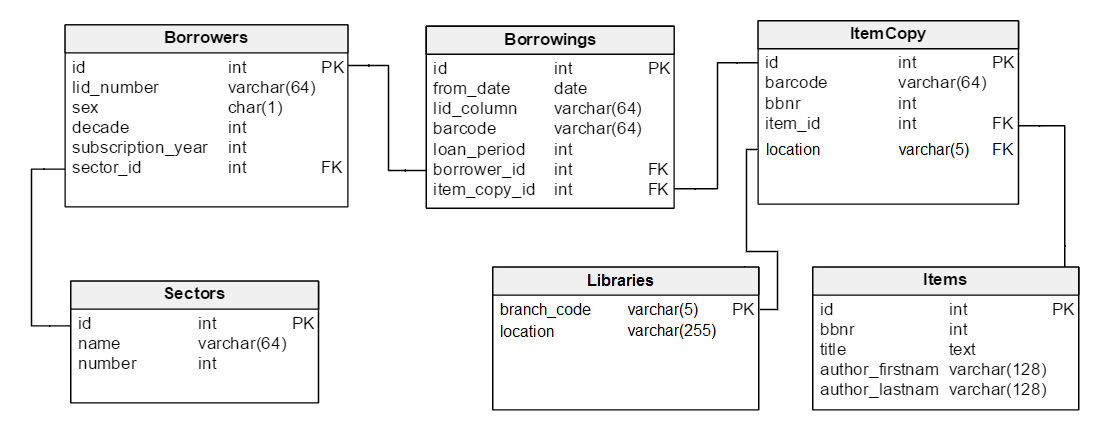
\includegraphics[width=16cm]{fig/db}
	\caption{Simplified database schema.}
	\label{fig:db}
\end{figure}

We make use of three main components in the backend.
First there is part responsible for importing the data consisting of a script in R that performs a cleanup of the CSV data provided by the Open Datatank and a script that imports this CSV into the database. The second component is the database, for which we will use PostgreSQL, a commonly used relational database  (Fig.~\ref{fig:db}). As last main component, we have the Django Web Framework. The blocks in this framework consist of an online and offline section. In the online section we have the REST-API which will be used to open up our data to our website and also towards other applications because of the open data concept. Besides this REST-API there is also a logical unit where the caching of requests, data,... will happen. At the offline section of the Django Web Framework, we will provide an import unit to put the data provided as CSV into our database. This is an offline block since the data is provided as a data dump and only needs to imported once. Since it will make use of the mapping that Django provides between the database and Python objects, it is included in the Django block.\\




\section{Functional requirements}

\subsection{User interface}

When the website will be loaded for the first time, at first an empty map of Ghent will be shown, together with one big number counting the sum of all books that were ever loaned at the library of Ghent. The map is divided in neighbourhoods. The shape of these sectors is static and will be shown on the map. Beneath the map, there will be a slider showing the time span in relation to the published data. Every sector can be selected, and if no selection is made, the data will be represented as it was for the whole area of Ghent.  On the website, you can select a neighourhood to query the neighbourhood for more specific information (amount of borrowers, amount of borrowings per person,...). Also different visualisations are possible so you can get a visualisation of certain properties like the amount of borrowings per person per neighbourhood.

\subsection{Linked Data}

We were requested by \emph{Pieter Colpaert} and \emph{Anastasia Dimou} to provide compatibility with a project they will set up at the main \emph{Apps for Ghent} event involving linked data. In order to provide this compatibility we would need to add context mappings using \emph{JSON-LD} to our data that is already provided as \emph{JSON}. In order to globally uniquely define an item such as a book, both teams need to decide on the same URI for a given item. For this reason, we would need to define the same mapping from the provided CSV to JSON-LD using the same RML mapping rules.

Although this is an interesting idea, we did not continue with it because of extra time that was lost cleaning up the data and switching from MongoDB to PostgreSQL and because Pieter and Anastasia did not continue with their project at \emph{Apps for Ghent}.

\subsection{API}

In order to provide data to the frontend and external services (such as linked data applications), an API has to be decided on. The aim of this section is to give an overview of the calls that can be made this API and the kind of data it will return.

\subsubsection{Root URL}

{\bf Usage}:
\begin{verbatim}
http://api.honegger.elis.ugent.be/v1/
\end{verbatim}

The API will be accessible through URLs that start with \texttt{http://api.honegger.elis.ugent.be/v1/}, where \texttt{v1} indicates the major version of the API. This version number is included so future versions of the API can deprecate certain parts without having to worry about external services breaking because of these changes.

\subsubsection{Items}

{\bf Usage}:
\begin{verbatim}
http://api.honegger.elis.ugent.be/v1/items/[?param_1=value_1]
  [&param_2=value_2]...[&param_n=value_n][/count]
\end{verbatim}

{\bf Parameters}:
\begin{itemize}
  \item \texttt{sector}: Identifier for the statistical sector. When provided, only items that were loaned by people living in the given sector will be returned.
  \item \texttt{age\_description}: Description of the target age of the item.
  \item \texttt{from\_date}: When provided, only items that were loaned after (and including) the given date are returned.
  \item \texttt{until\_date}: When provided, only items that were loaned before (and including) the given date are returned.
  \item \texttt{limit}: The maximum number of items that should be returned.
  \item \texttt{order}: A comma-seperated list of properties on which to sort the data in ascending order. Descending order can be achieved by adding a $-$ before the property.
\end{itemize}

The main resources that are provided by the API are \emph{items} present in the library, such as \emph{books} and \emph{DVDs}.
By calling the URL listed above, a list of \emph{items} can be fetched that can be filtered using various optional parameters.
The return value should be a list of \emph{items} containing their unique identifiers, various metadata properties (such as title, genre, theme, ...), the library the item was loaned from and the number of times the items was loaned, given the parameters.\\

Because the main visualisation can get away with only the number of loans for all items given a set of parameters, an extra \texttt{/count} action can be used, which simply returns the number of loans instead of a list of items.

\section{Use case}

The library personel can use the web application in two ways, reactively and pro-actively. Respectively by searching on a specific book (title) or on a certain group of books (genre, target-age,...) and otherwise looking for differences between the current distribution (visualised per library) and the preffered distribution (visualised per sector). If the demand of a certain book is skewed for a sector, the copies can be moved closer (towards the library with the least distance) to this sector. If the demand of a group correlates with a sector the personel can decide to anticipate onto the demand of similar books in this group and move these books closer to the specified group.\\

The data that is however provided by the library does not give us the possibility to continue with the whole use case. We will however be able to show a with some interesting properties per sector, for which the data is fetched from our API. The querying for books,... is not possible anymore since no location data is given from the library spots.
